 %%%%%%%%%%%%%%%%%%%%%%%%%%%%%%%%%%%%%%%%%
% University Assignment Title Page 
% LaTeX Template
% Version 1.0 (27/12/12)
%
% This template has been downloaded from:
% http://www.LaTeXTemplates.com
%
% Original author:
% WikiBooks (http://en.wikibooks.org/wiki/LaTeX/Title_Creation)
%
% License:
% CC BY-NC-SA 3.0 (http://creativecommons.org/licenses/by-nc-sa/3.0/)
% 
% Instructions for using this template:
% This title page is capable of being compiled as is. This is not useful for 
% including it in another document. To do this, you have two options: 
%
% 1) Copy/paste everything between \begin{document} and \end{document} 
% starting at \begin{titlepage} and paste this into another LaTeX file where you 
% want your title page.
% OR
% 2) Remove everything outside the \begin{titlepage} and \end{titlepage} and 
% move this file to the same directory as the LaTeX file you wish to add it to. 
% Then add \documentclass[12pt]{article}
\usepackage[english]{babel}
\usepackage{amsmath}
\usepackage{graphicx}
\usepackage{textcomp}
\usepackage{parskip}
\usepackage[colorinlistoftodos]{todonotes}
\usepackage{csquotes}
\usepackage{float}
\usepackage[backend=biber,style=ieee]{biblatex}
\addbibresource{bibliography.bib}

\begin{document}

\begin{titlepage}

\newcommand{\HRule}{\rule{\linewidth}{0.5mm}}
\center 

\textsc{\LARGE Iowa State University }\\[1.5cm] 
\textsc{\Large Center for Statistics and Applications in Forensic
Evidence
}\\[0.5cm] 

\HRule \\[0.4cm]
{ \huge \bfseries Shoe Print Data Collection: Additional Methods }\\[0.4cm] 
\HRule \\[1.5cm]



\begin{center}
\centering
 
\includegraphics[scale=.4]{csafe-logo}\\[1cm]
\end{center}







\end{titlepage}

\section{Introduction}

 When developing the methodology for the longitudinal shoe study conducted by the Center for Statistics and Applications in Forensic Evidence (CSAFE), collection procedures were designed to obtain the most ideal shoe-sole impression possible. While these images will be useful to the researcher and practitioner communities, they do not provide realistic examples of prints that would be collected from a crime scene/suspected crime scene. For this reason, CSAFE researchers have compiled this manual which contains procedures for further data collection and offers new, or edited, procedures that better represent the practices of current forensic examiners and crime scene teams. If at any time there is a question on any of these procedures, please make a note using a post-it note and e-mail the principal investigator, the project manager, the faculty in charge of the study, or the author of the specific procedure. 

\end{document} to your LaTeX file where you want your
% title page.
%
%%%%%%%%%%%%%%%%%%%%%%%%%%%%%%%%%%%%%%%%%
%\title{Description of Outsole Impression Methods}
%----------------------------------------------------------------------------------------
%	PACKAGES AND OTHER DOCUMENT CONFIGURATIONS
%----------------------------------------------------------------------------------------

\documentclass[12pt]{article}
\usepackage[english]{babel}
\usepackage[utf8x]{inputenc}
\usepackage{amsmath}
\usepackage{graphicx}
\usepackage[colorinlistoftodos]{todonotes}

%% Forcing images to stay in their corresponding section
\usepackage{placeins}
\let\Oldsection\section
\renewcommand{\section}{\FloatBarrier\Oldsection}
\let\Oldsubsection\subsection
\renewcommand{\subsection}{\FloatBarrier\Oldsubsection}
\let\Oldsubsubsection\subsubsection
\renewcommand{\subsubsection}{\FloatBarrier\Oldsubsubsection}


% Set images path
\graphicspath{ {images/} }

% Links to sections.
\usepackage{hyperref}

\begin{document}

\begin{titlepage}

\newcommand{\HRule}{\rule{\linewidth}{0.5mm}} % Defines a new command for the horizontal lines, change thickness here

\center % Center everything on the page
 
%----------------------------------------------------------------------------------------
%	HEADING SECTIONS
%----------------------------------------------------------------------------------------
\textsc{\LARGE Iowa State University}\\[1.5cm] % Name of your university/college
\textsc{\large Center for Statistics and Applications in Forensic Evidence }\\[0.5cm] % Minor heading such as course title

%----------------------------------------------------------------------------------------
%	TITLE SECTION
%----------------------------------------------------------------------------------------

\HRule \\[0.4cm]
{ \huge \bfseries Dental Stone Shoe Sole Casting: Procedure}\\[0.4cm] % Title of your document
\HRule \\[1.5cm]
 
%----------------------------------------------------------------------------------------
%	AUTHOR SECTION
%----------------------------------------------------------------------------------------
\begin{minipage}{0.4\textwidth}
\begin{flushleft} \large
\emph{Author:}\\
Jenny Kim, \newline Benjamin Wonderlin, and James \textsc{E. Kruse, } % Your name
\end{flushleft}
\end{minipage}
~
\begin{minipage}{0.4\textwidth}
\begin{flushright} \large
\emph{Principal Investigator:} \\
 \textsc{Dr. Guillermo Basulto-Elias, and Dr. Susan Vanderplas } % Supervisor's Name
\end{flushright}
\end{minipage}\\[2cm]

% If you don't want a supervisor, uncomment the two lines below and remove the section above
%\Large \emph{Author:}\\
%John \textsc{Smith}\\[3cm] % Your name
%----------------------------------------------------------------------------------------
%	LOGO SECTION
%----------------------------------------------------------------------------------------


\includegraphics[scale=.5]{Logo}\\[1cm]

\begin{center}
\begin{tabular}{ c   |   c } 
 
\end{tabular}
\end{center}
%----------------------------------------------------------------------------------------
%	DATE SECTION
%----------------------------------------------------------------------------------------

{\large \today}\\[2cm] % Date, change the \today to a set date if you want to be precise


 
%----------------------------------------------------------------------------------------

\vfill % Fill the rest of the page with whitespace

\end{titlepage}
 
\tableofcontents

\newpage

\section{Introduction}

The following is the recommended procedure for using dental stone to cast shoe out-sole prints that have been found/taken in mud/dirt. The specific stone used in this procedure is Dent Stone. While it is not the primary purpose of this material, it is commonly used by forensic professionals when creating casts of shoe impressions found in mud, sand, and snow. 

\subsection{Building The Drainage Apparatus}

1. Obtain three 49.29L, flat, under-bed storage totes. Using a hand held drill, evenly distribute drainage holes on the bottom surface of one storage tote.

\begin{figure}[!htp]
\centering
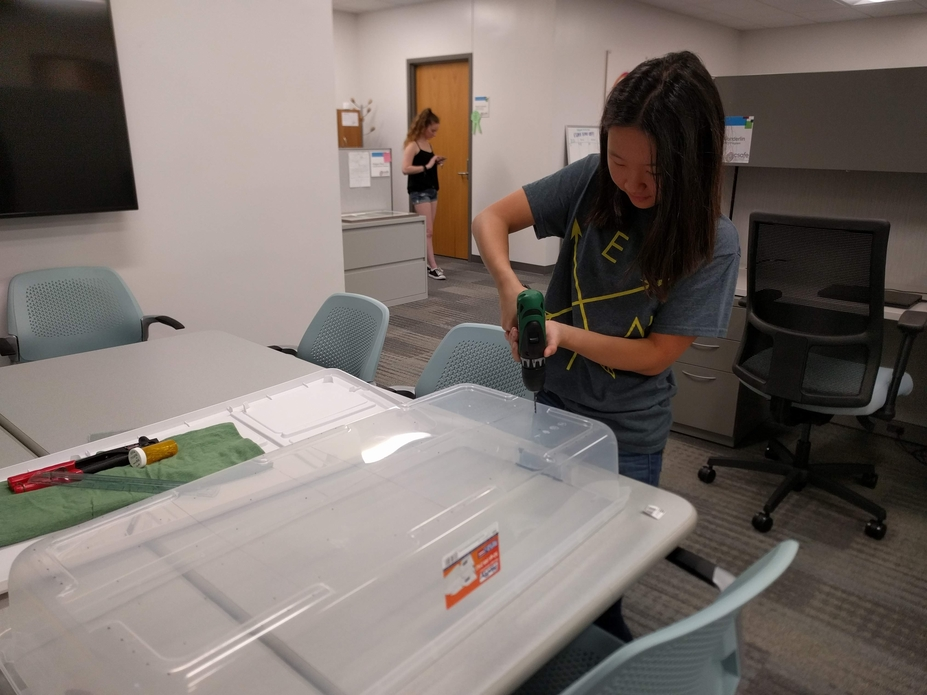
\includegraphics[width=5cm]{Cast_Drill}
\caption{Drilling holes into the bin will allow water to drain out of the apparatus}
\label{Image 1}
\end{figure}

2.Place 3-7, depending on size, pieces of wood along the inside surface of a second tote. Lay the tote from step one on top of the wood.This is meant to provide support once the weight of an adult body is placed on the apparatus. Once well aligned, attach the wood to the tote from step one. 

3. Line the tote from step one with a pillowcase such that the entire inside surface is covered. This will act as a filter and keep the dirt/mud in the tote. Attach the pillowcase using a rivet gun, making sure that the edges are high enough that dirt/mud will not escape the filter. 

4. Place tote 1 into tote 2. Fill the lined tote and third remaining tote with equal amounts of dirt. The dirt should not surpass the upper edge of the pillowcase in the lined tote.

\subsection{Soil Preparation: Damp Soil} 

1. Scoop a 2 cup sample of dirt into a 1-gallon plastic bag. 

2. Turn on and zero a standard kitchen scale. Weigh the Ziploc bag on the scale. For reference, the 1-gallon Ziploc alone should weigh about 17g.

3. Add room-temperature water to the bag in small, measured intervals until the soil is of the desired consistency. The final weight of the 2 cup sample should be 490 grams. 

4. Use the amount of water added to the sample to estimate the amount of water necessary for the soil tub. Pour the estimated amount of water evenly across the soil tub remembering that is easy to add water but difficult to remove it if the soil becomes too saturated. 

5. Mix until the soil is homogeneous. Take another 2 cup sample to make sure that the soil is at the correct saturation level. 2 cups should weigh 490 grams. 

\subsection{Soil Preparation: Mud at Field Capacity} 

1. Evenly pour water over the soil until a steady stream of water drains below. 

2. Mix the mud by hand until the mixture is homogeneous. Wait for the bin to finish draining before stepping in the mud. 

\subsection{Creating Realistic Shoe Out-sole Prints}

1. Place the filled totes parallel to each other. A smaller bin should be placed at an end of the drainage tote to receive the muddy shoes. Leave enough room for the tripod to maneuver between the two stations.

2. One technician will put on the shoes and take three, natural, steps though the dry dirt bin. 

3. This procedure will be repeated for the mud bin (Figure 2). 

\begin{figure}[!htp]
\centering
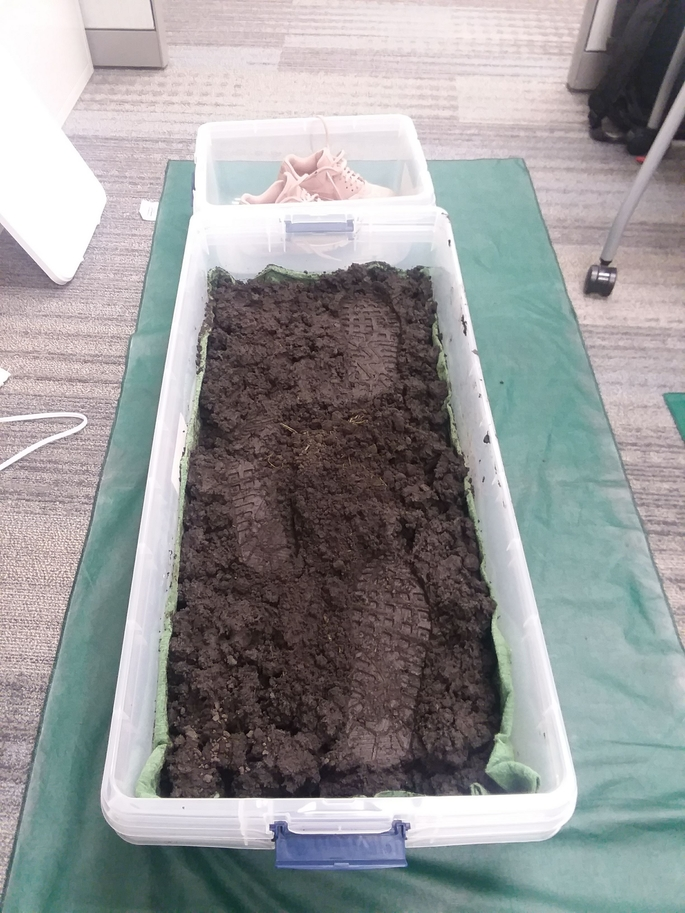
\includegraphics[width=5cm]{Cast_Bin}
\caption{The Technician will take three natural steps through the mud. }
\label{Image 2}
\end{figure}

\subsection{Shoe Impression Photography and scanning}

1. Place the L-shaped ruler next to the shoe print such that the heel of the shoeprint is open.

2. Photograph all prints in high definition. Place and level a tripod next to the print. Position the tripod arm about 2 feet above the print. Firmly fasten the camera on to the arm and use a bubble level to level  the arm. It may be necessary to raise or lower certain legs of the tripod to achieve balance. Fasten a counterweight (approximately 8 extra sheets of linoleum flooring in the tripod bag will suffice) along the back of the tripod. Please reference the high resolution photography procedure for exact tripod and camera set-up. 

3.  Locate the attachment point on the end of the tripod arm. Making sure that the counter weight is present on the backside of the tripod, press the orange button and slide the camera into place. There will be a small click when the camera is in place. 

4. Making sure that the camera is turned off, plug the USB cable into the camera body (left side). Do not force the plug or the screw into the camera. Plug the other end into the back of the laptop. 

5. Remove the lens cap and turn on the camera by sliding the switch located on the upper left-hand side of the camera from Off to On

6. The computer currently opens the following:
•	Control panel/hardware and sound/devices and printers/canon EOS 5d mark IV
i.	this window can be closed
•	EOS utility 3
ii.	if this program does not start you can manually start it

7. To remotely take pictures, select “remote shooting”

8. The pop up that comes up is used to control the camera. Select “live view” on this same menu

9. Make sure that the ruler is flat and not covering any portion of the print. 

10. Now, using the live view on the laptop, make sure that the shoe impression and the scale are both present in the shot. If all is visible on the screen, press the acquire button on the main control menu (Figure 3). 

\begin{figure}[!htp]
\centering
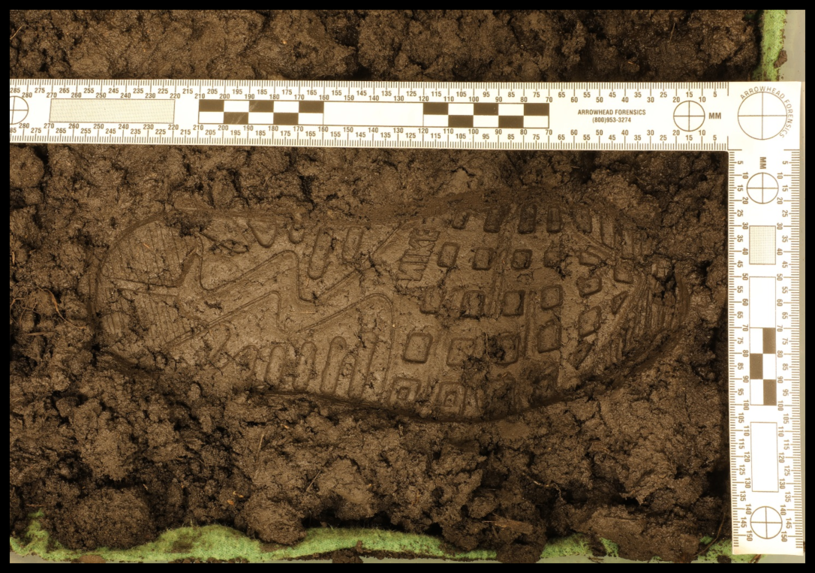
\includegraphics[width=6cm]{CastPhoto2}
\caption{Sample of a good photo }
\label{Image 3}
\end{figure}

11. Properly name and save the image to the desired folder on the desktop or shared drive. 

12. Take a second image, but this time, utilize the night stick to illuminate the impression from the right side. 

13. Take a third image, but this time, utilize the night stick to illuminate the impression from the left side (Figure 4). At this point, remove the scale and put away the camera and tripod.  

\begin{figure}[!htp]
\centering
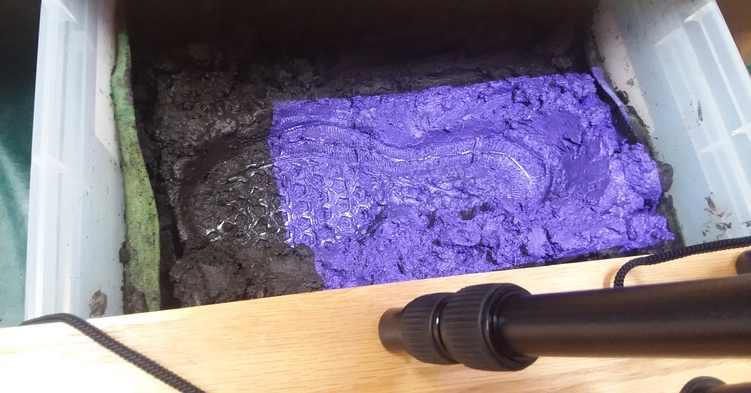
\includegraphics[width=8cm]{BoardScan}
\caption{Light the photo from both the left and right sides.}
\label{Image 4}
\end{figure}

\newpage

14. Following the 3D Scanning procedure for soil, take two scans of each impression that is being casted. Properly name and save the resulting model to the desired folder on the desktop or shared drive (Figure 5). 

\begin{figure}[!htp]
\centering
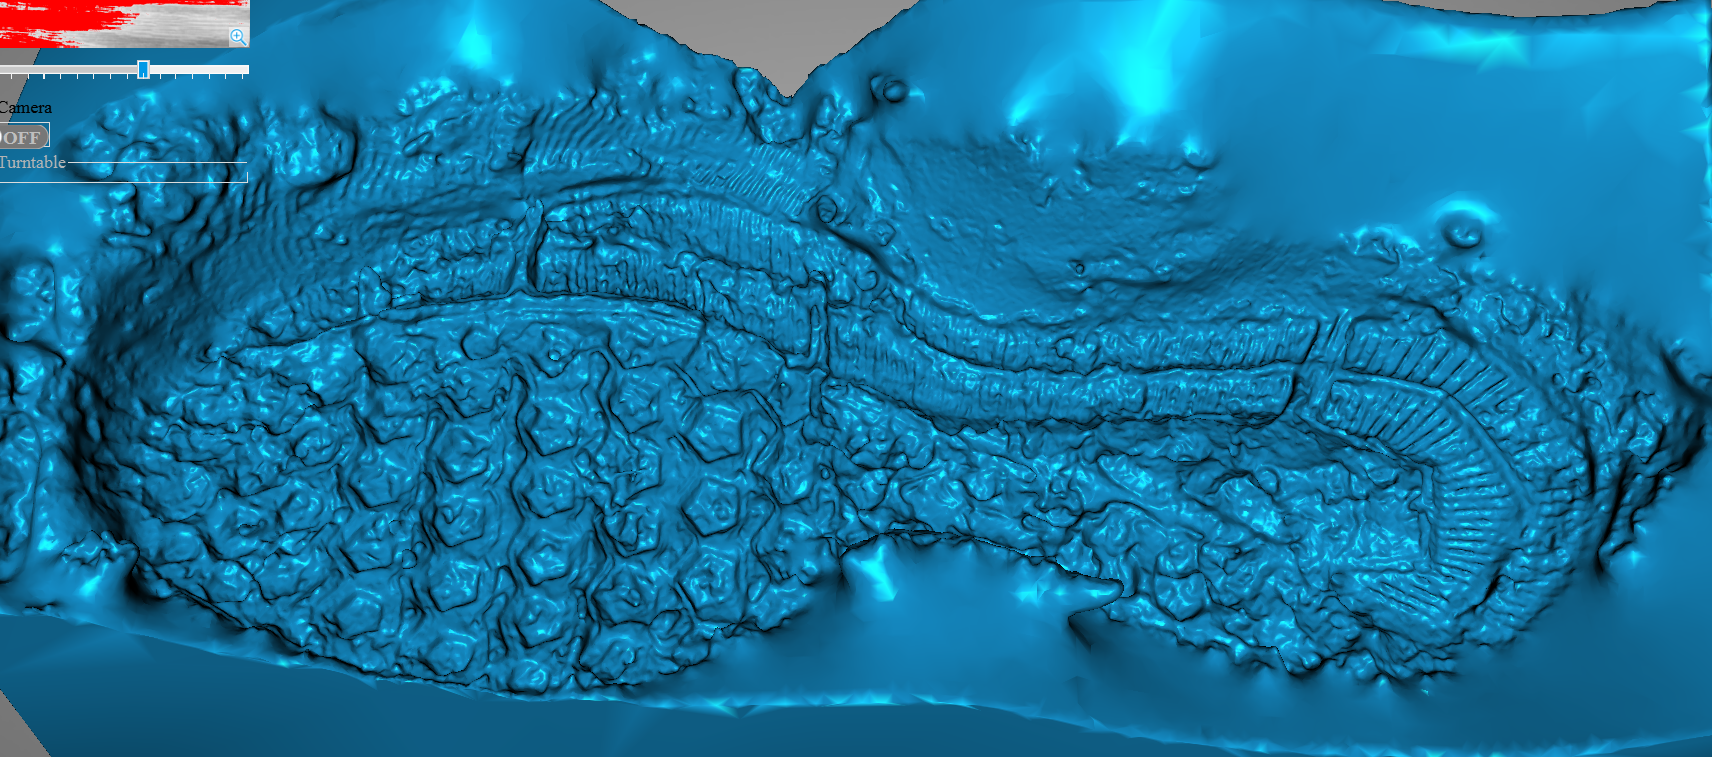
\includegraphics[width=8cm]{Capture3}
\caption{After photos have been taken, 3D scan the impression. }
\label{Image 5}
\end{figure}

\subsection{Pouring Shoe out-sole Casts}

1. Evenly spray the print with a silicone release agent or hairspray. Make sure to hold the can roughly 31 cm from the impression. 

2. If needed, place a frame around the perimeter of the print, leaving about a half inch gap between the print and the frame. For inclines, build up the lower portions of the impression with rock, mud, or dirt. Make sure that any alterations to the area do not disturb the impression. 

3. Scoop out 900 grams of dental stone into a ziploc bag(Figure 6).

\begin{figure}[!htp]
\centering
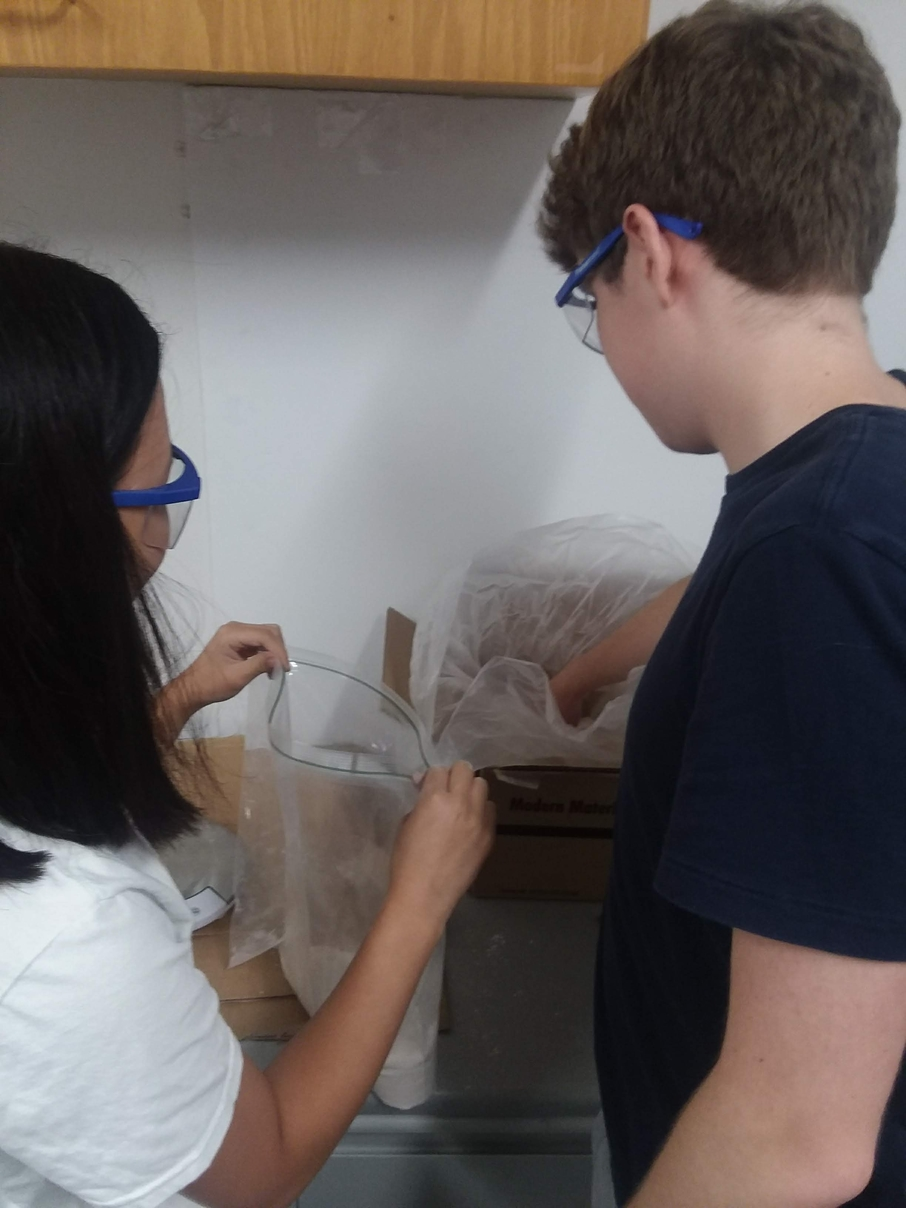
\includegraphics[width=5cm]{Cast_Scoop}
\caption{Portion out the correct amount of dry stone powder into a gallon ziploc bag}
\label{Image 6}
\end{figure}

\newpage

4. Pour 325 ml of room-temperature water into the 1-gallon plastic bag. It is best to add the water in small increments to prevent an undesired consistency. For reference, the water/powder ratio is 22 ml/100 gm. 

5. Seal the plastic bag and use hands to mix the powder and water until it reaches the consistency of thick pancake batter. Mix quickly (Figure 7).

\begin{figure}[!htp]
\centering
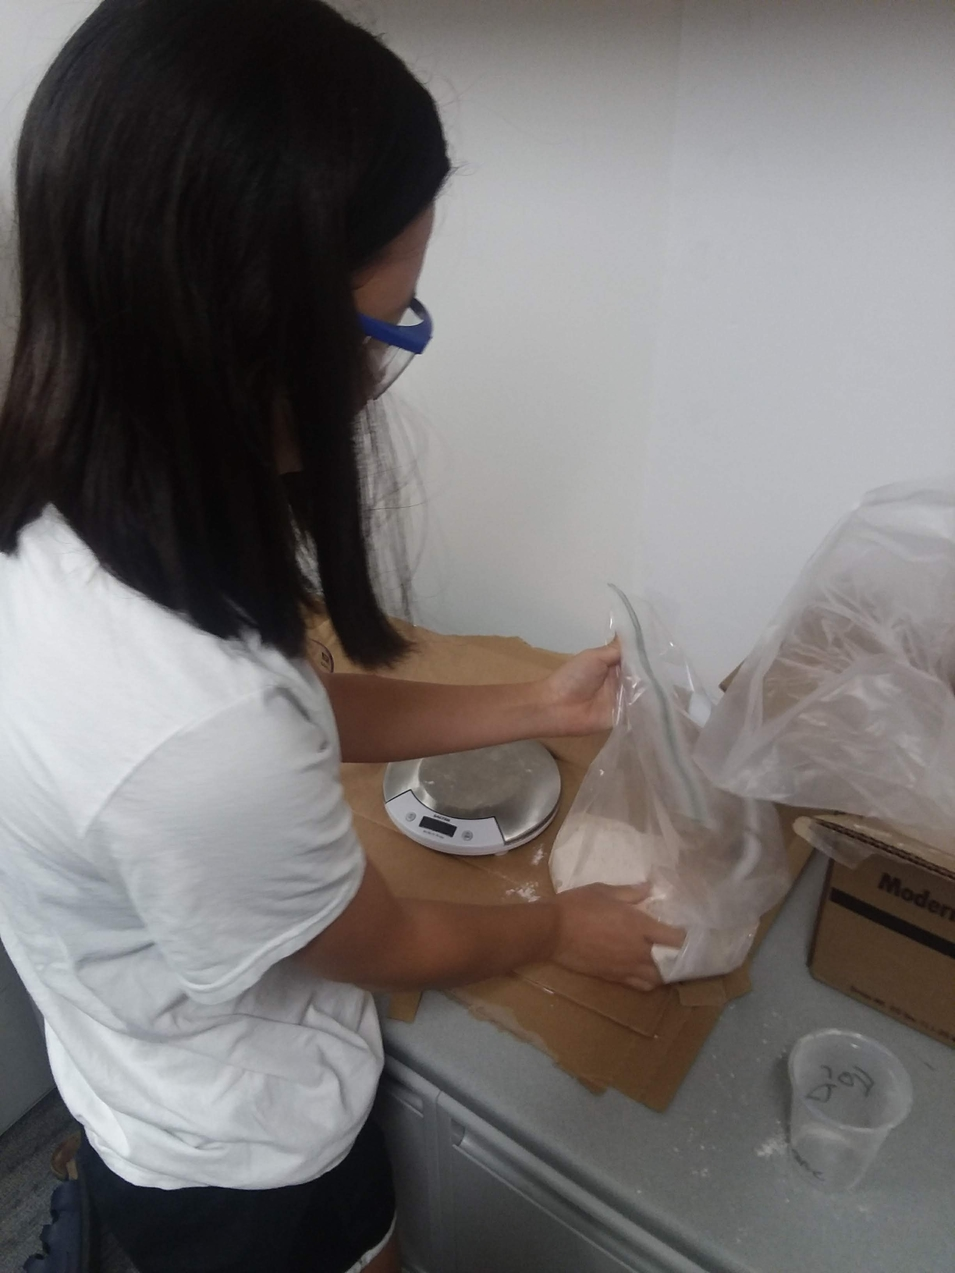
\includegraphics[width=5cm]{Cast_Mix}
\caption{As soon as the water has been added, quickly start mixing}
\label{Image 7}
\end{figure}

\newpage

6. Immediately cut off a corner of the plastic bag and slowly pour the dental stone according to one of the following methods:
\begin{itemize}
\item Pour around the perimeter of the impression, allowing the dental stone to flow inwards.
\item Recommended: Dig a small funnel along the perimeter of the print. Pour the dental stone into the funnel until the the entire impression is covered (Figure 8).
\end{itemize}

\begin{figure}[!htp]
\centering
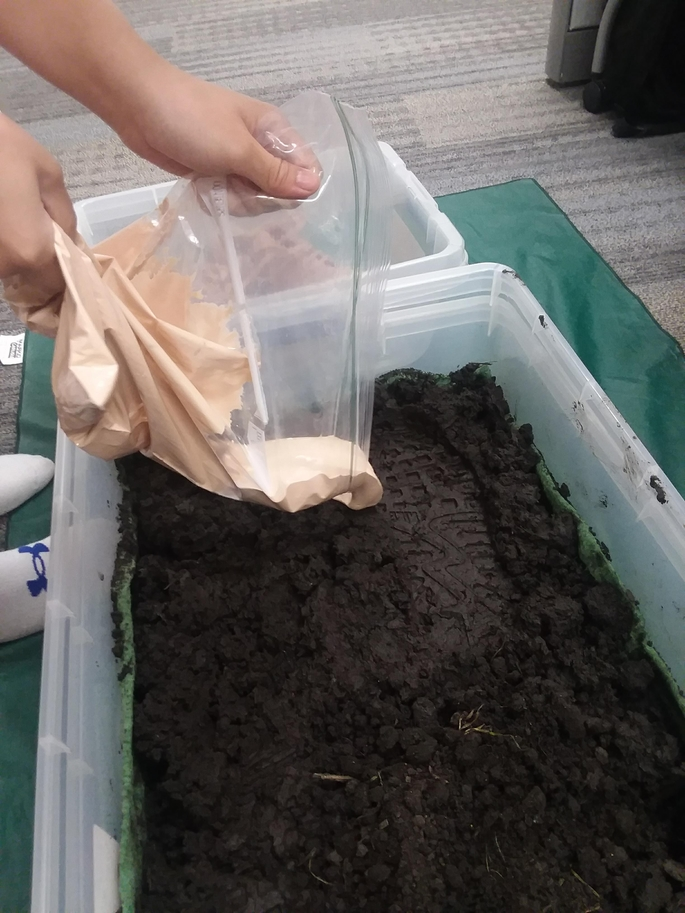
\includegraphics[width=5cm]{Cast_Pour}
\caption{Pour dent stone into a small, dirt, funnel and not onto the print itself.}
\label{Image 8}
\end{figure}

\newpage

7. Once the impression is filled to a depth of approximately 1 inch, a piece of cardboard can be used to gently spread the mixture evenly on the surface.

8. Allow the cast to dry for 30 minutes (Figure 9). Longer drying periods should be considered to account for low temperatures, larger impressions, wetter casting materials, and high ground moisture content.

\begin{figure}[!htp]
\centering
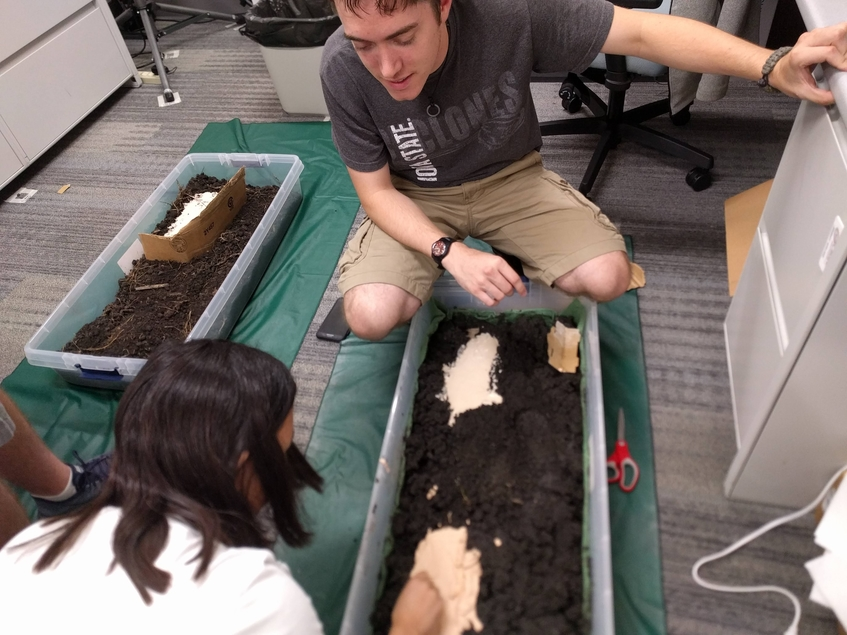
\includegraphics[width=5cm]{Cast_Set}
\caption{Allow the cast to dry for 30-60 min.}
\label{Image 9}
\end{figure}

9. Label the print appropriately by gently engraving letters into the shoe print with a paperclip. If already dry, use a permanent marker.

\subsection{Removal, Cleaning, and Storage of Casts}

1. Remove the cast manually by digging deeply around the perimeter of the impression. Use both hands to evenly pull from underneath of the cast (Figure 10).

\begin{figure}[!htp]
\centering
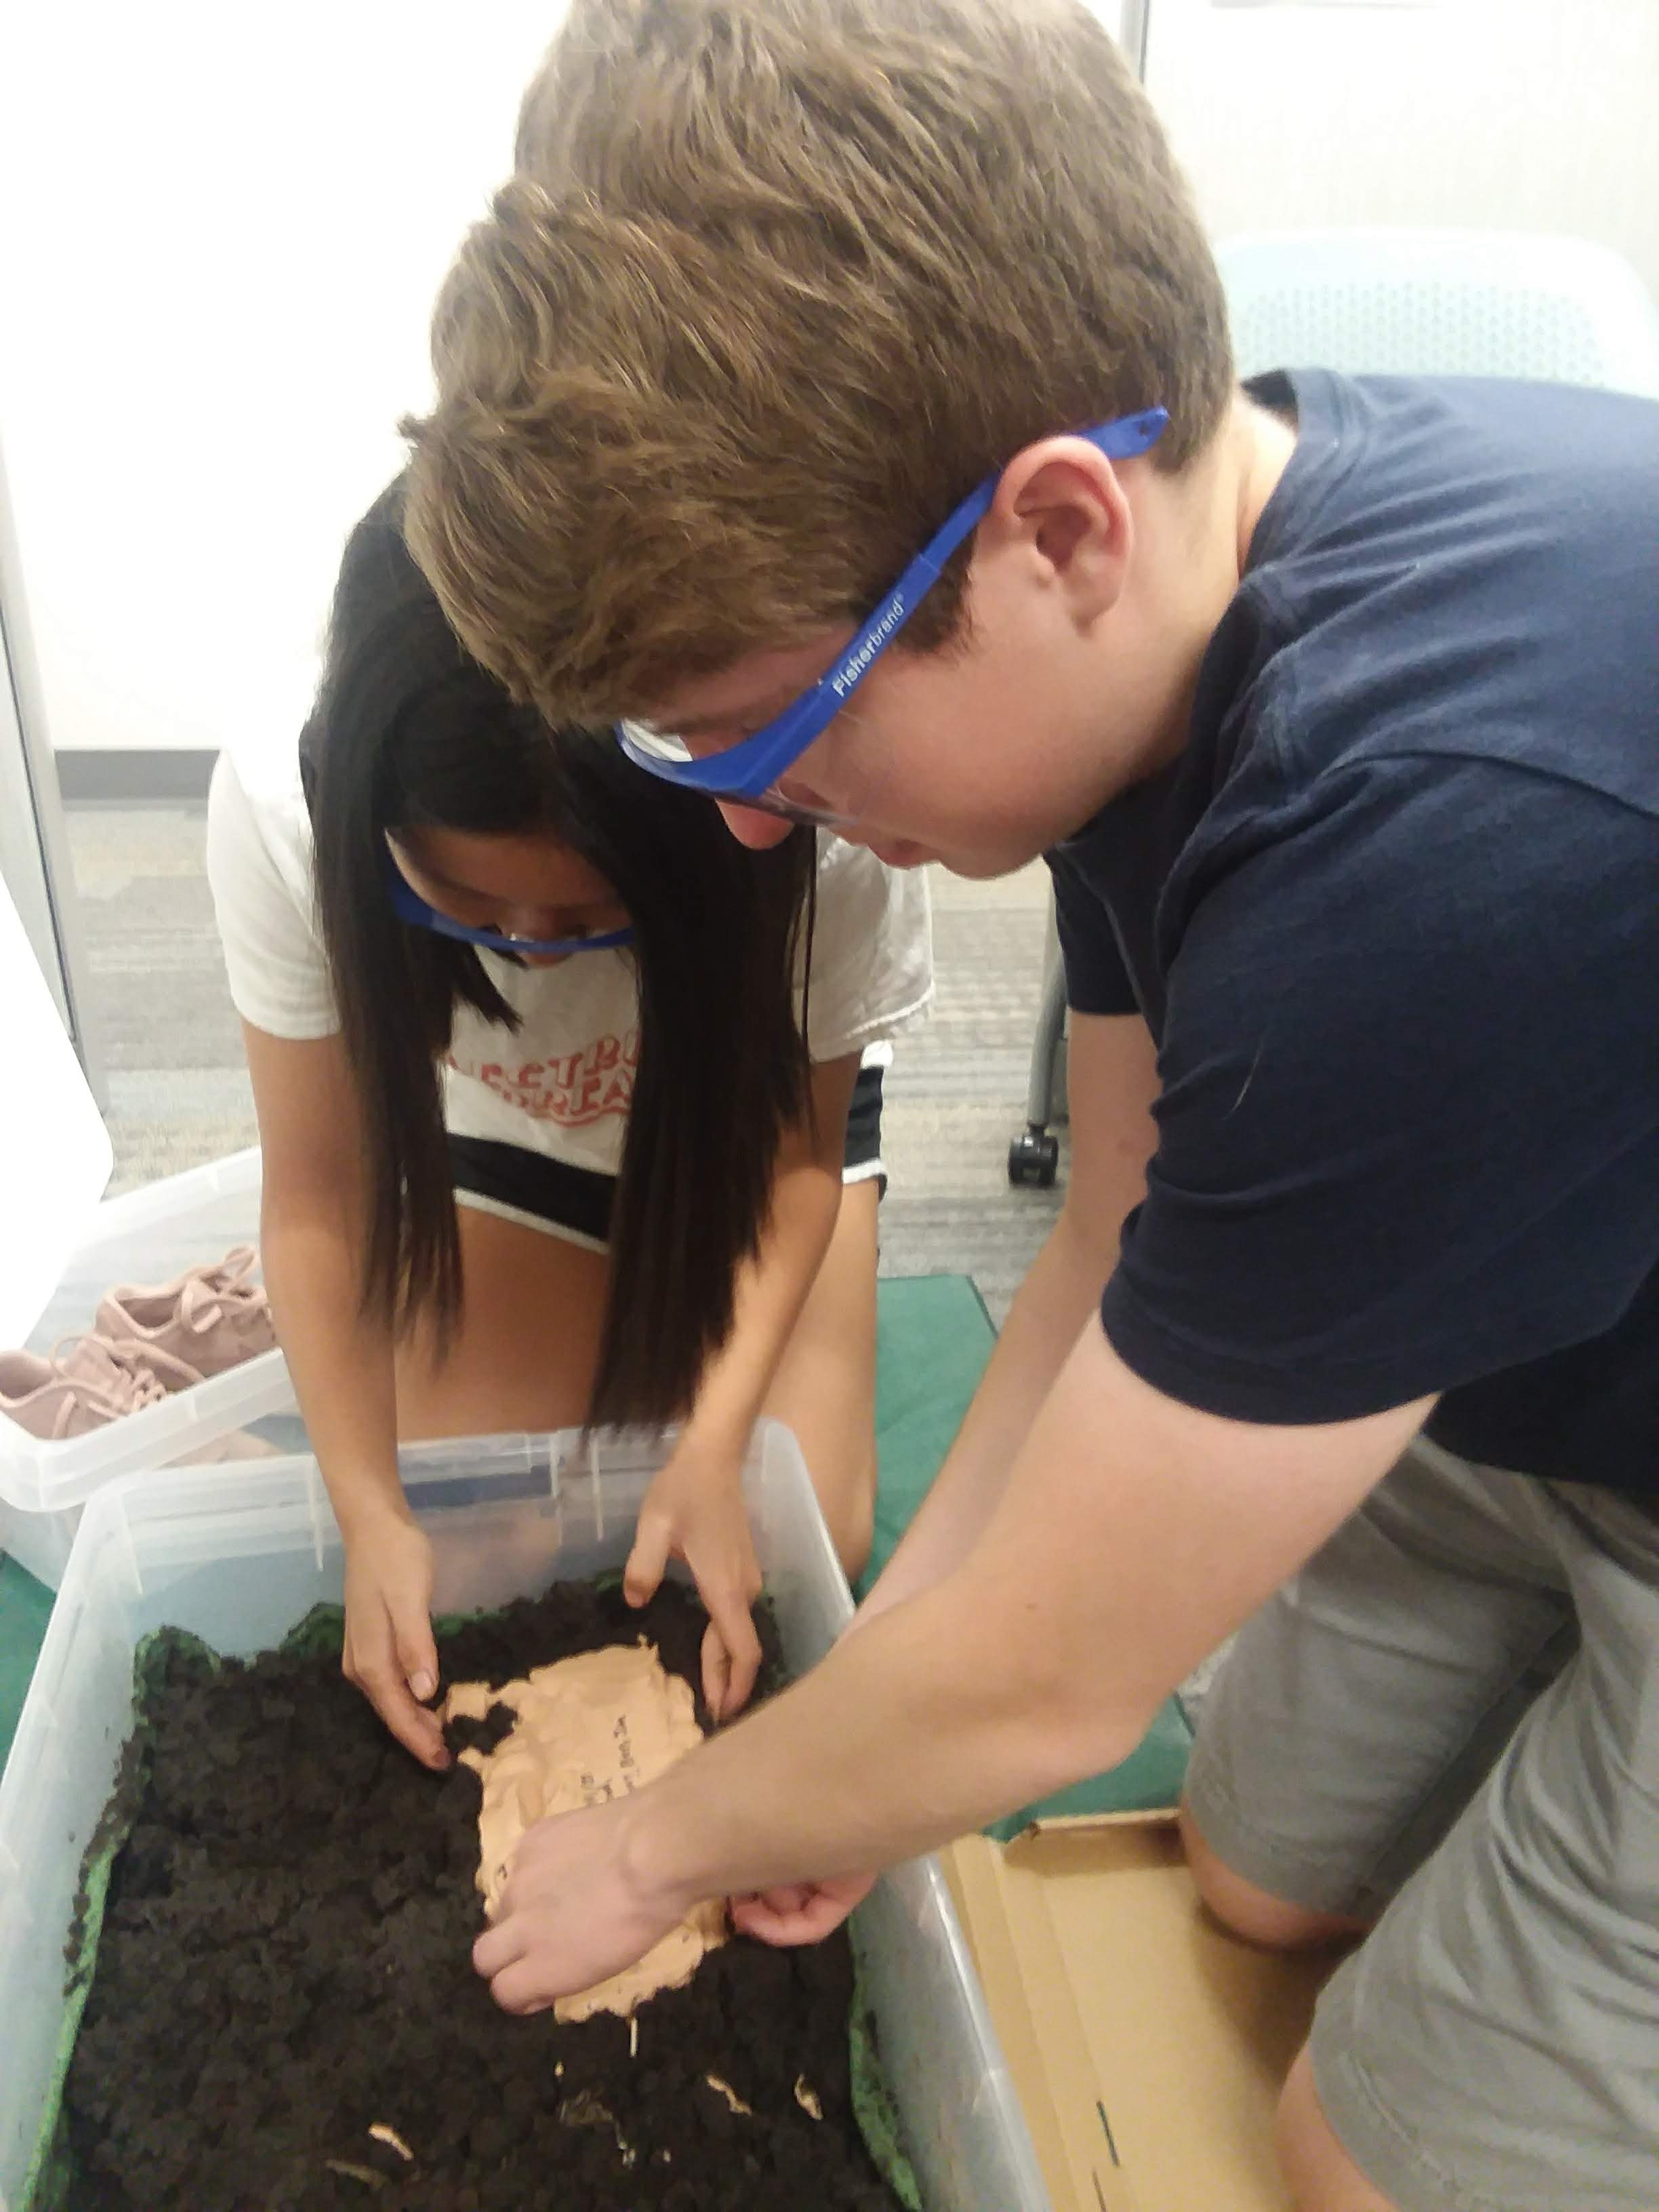
\includegraphics[width=5cm]{Cast_done}
\caption{Carefully remove the cast from the dirt. }
\label{Image 10}
\end{figure}

2. Leave the cast to sit and air out on cardboard for a 48-hour period.

3. Hold cast under running water and scrub the dirt using circular motions with a soft bristled brush.



\end{document}

